\chapter{Présentation du projet et cahier des charges}
\label{chap:projet}

\section{Introduction}

Avant toute réalisation technique, il est essentiel de définir le cadre général du projet, ses objectifs, les besoins à satisfaire et la méthode à suivre. Le cahier des charges constitue la base du travail en précisant les aspects fonctionnels, organisationnels et techniques qui orienteront la suite du projet. Dans le cadre du \textbf{projet PACTE}, il permet d'identifier les attentes liées au sujet, de les traduire en exigences concrètes et de déterminer les contraintes à respecter. Ce chapitre présente donc le projet, sa problématique, ses objectifs, son périmètre, les besoins fonctionnels et non fonctionnels ainsi que la méthodologie et le planning prévisionnel.

\section{Présentation et contexte}

Ce projet a pour objectif de concevoir un système capable de reconnaître, à partir de l'image d'un objet, six usagers de la route : la \textbf{personne}, le \textbf{vélo}, la \textbf{voiture}, la \textbf{moto}, le \textbf{bus} et le \textbf{camion}. Pour chaque image, le modèle renvoie une classe ainsi qu'un \textbf{score de confiance}. Une fois entraîné, il est testé sur des images qu'il n'a jamais vues, puis utilisé par un véhicule virtuel qui circule dans les vraies rues de Casablanca.

Le projet place l'équipe dans la position d'une cellule de développement chargée de mettre en œuvre la brique de perception d'un véhicule autonome. Notre équipe est composée de trois étudiants, chacun étant responsable d'un rôle précis.

\begin{table}[H]
\centering
\caption{Répartition des rôles au sein de l'équipe}
\label{tab:roles}
\begin{tabularx}{\textwidth}{>{\raggedright\arraybackslash}p{3.8cm}>{\raggedright\arraybackslash}p{3.6cm}Y}
  \toprule
  \entete \textbf{Rôle} & \textbf{Responsable} & \textbf{Missions} \\
  \midrule
  Données & \acompleter{Nom} & Exploration, prétraitement, recadrages et découpage des données \\
  Modèles & \acompleter{Nom} & Extraction des caractéristiques, entraînement des classifieurs et suivi des essais \\
  Évaluation et intégration & \acompleter{Nom} & Évaluation finale, analyse des erreurs, export du modèle et lien avec le simulateur \\
  \bottomrule
\end{tabularx}
\end{table}

\section{Problématique}

Dans la plupart des systèmes de conduite autonome, la reconnaissance des usagers de la route repose sur des modèles très volumineux, entraînés sur des millions d'images et sur des machines puissantes. Dans un cadre académique, avec un \textbf{jeu de données de taille limitée}, \textbf{sans poids préentraînés} et \textbf{sans GPU dédié}, la question de la fiabilité d'un tel modèle se pose naturellement.

Le projet AutoMaze AI vise à répondre à la question suivante :

\begin{quote}
\itshape Un modèle entraîné de zéro sur un jeu de données de taille limitée peut-il reconnaître les usagers de la route de manière suffisamment fiable pour guider les décisions d'un véhicule autonome virtuel ?
\end{quote}

De cette question découlent trois interrogations complémentaires. Il s'agit d'abord de déterminer quel classifieur, parmi SVM, Random Forest et k-NN, obtient les meilleurs résultats sur les mêmes caractéristiques. Il faut ensuite identifier les classes les plus difficiles à reconnaître et comprendre pourquoi. Enfin, il est important de mesurer les conséquences d'une erreur du modèle sur le comportement du véhicule, notamment lorsqu'un piéton n'est pas reconnu.

\section{Objectifs du projet}

\subsection{Objectif général}

L'objectif principal du projet est de \textbf{développer et d'évaluer un classifieur d'objets routiers entraîné de zéro}, puis de montrer comment ses prédictions peuvent guider un \textbf{véhicule autonome virtuel} jusqu'à sa destination.

\subsection{Objectifs spécifiques}

Pour atteindre cet objectif général, plusieurs objectifs spécifiques ont été définis :

\begin{table}[H]
\centering
\caption{Objectifs spécifiques et mesures de réussite}
\begin{tabularx}{\textwidth}{l>{\raggedright\arraybackslash}p{5.8cm}Y}
  \toprule
  \entete \textbf{N°} & \textbf{Objectif spécifique} & \textbf{Mesure de réussite} \\
  \midrule
  OS1 & Décrire le jeu de données retenu & Provenance, volume, répartition par classe, résolution et qualité documentées \\
  OS2 & Préparer les images & Nettoyage, recadrage, normalisation et découpage sans fuite de données \\
  OS3 & Comparer SVM, Random Forest et k-NN & Accuracy, précision, rappel, F1 et matrice de confusion, calculés sur les mêmes données \\
  OS4 & Analyser les classes difficiles & Paires de classes confondues et images mal classées expliquées \\
  OS5 & Prédire la classe de nouvelles images & Affichage du type \og Image \textrightarrow{} Voiture (92~\%) \fg{} \\
  OS6 & Intégrer le modèle au véhicule virtuel & Chaque prédiction déclenche une décision, et les erreurs graves sont comptées \\
  \bottomrule
\end{tabularx}
\end{table}

Pour juger nos modèles, nous retenons principalement le \textbf{F1 macro}, qui accorde le même poids à chaque classe. Aucune valeur cible n'est fixée à l'avance : la référence sera le meilleur modèle classique, comparé à des scores planchers (section~\ref{sec:metriques}).

\section{Périmètre fonctionnel}
\label{sec:perimetre}

Afin d'éviter que le projet ne devienne trop vaste, nous distinguons les \textbf{fonctionnalités principales}, qui relèvent du Machine Learning et constituent le cœur scientifique du projet, des \textbf{fonctionnalités d'intégration}, qui servent à la démonstration finale.

\begin{table}[H]
\centering
\caption{Délimitation du périmètre par module}
\begin{tabularx}{\textwidth}{>{\raggedright\arraybackslash}p{3.4cm}Y>{\raggedright\arraybackslash}p{2.4cm}}
  \toprule
  \entete \textbf{Module} & \textbf{Responsabilité} & \textbf{Importance} \\
  \midrule
  Dataset & Fournir les images des objets routiers & Essentielle \\
  Prétraitement & Préparer les images pour l'apprentissage & Essentielle \\
  Classification ML & Identifier la classe d'un objet & Essentielle \\
  Évaluation & Comparer les classifieurs & Essentielle \\
  \midrule
  Simulateur & Fournir un environnement de démonstration & Intégration \\
  Localisation & Fournir les coordonnées des objets & Intégration \\
  Planification & Calculer le chemin le plus court & Intégration \\
  Décision & Choisir le comportement face aux obstacles & Intégration \\
  Contrôle & Commander le véhicule virtuel & Intégration \\
  \bottomrule
\end{tabularx}
\end{table}

Les fonctionnalités d'intégration sont nécessaires à la démonstration, mais nous veillerons à ce qu'elles ne prennent pas le dessus sur les expérimentations de Machine Learning demandées par le sujet.

\textbf{La détection d'objets reste hors périmètre.} Notre modèle ne recherche pas la position des objets dans une image complète, ce qui relèverait d'un détecteur comme YOLO ou R-CNN (figure~\ref{fig:detection}), interdit par les règles du cours. Il reçoit l'image d'un objet déjà isolé et en détermine la nature. Dans le simulateur, c'est la position connue de chaque objet qui remplace l'étape de détection. La vidéo et la physique réaliste du véhicule sont également exclues du périmètre.

\begin{figure}[H]
  \centering
  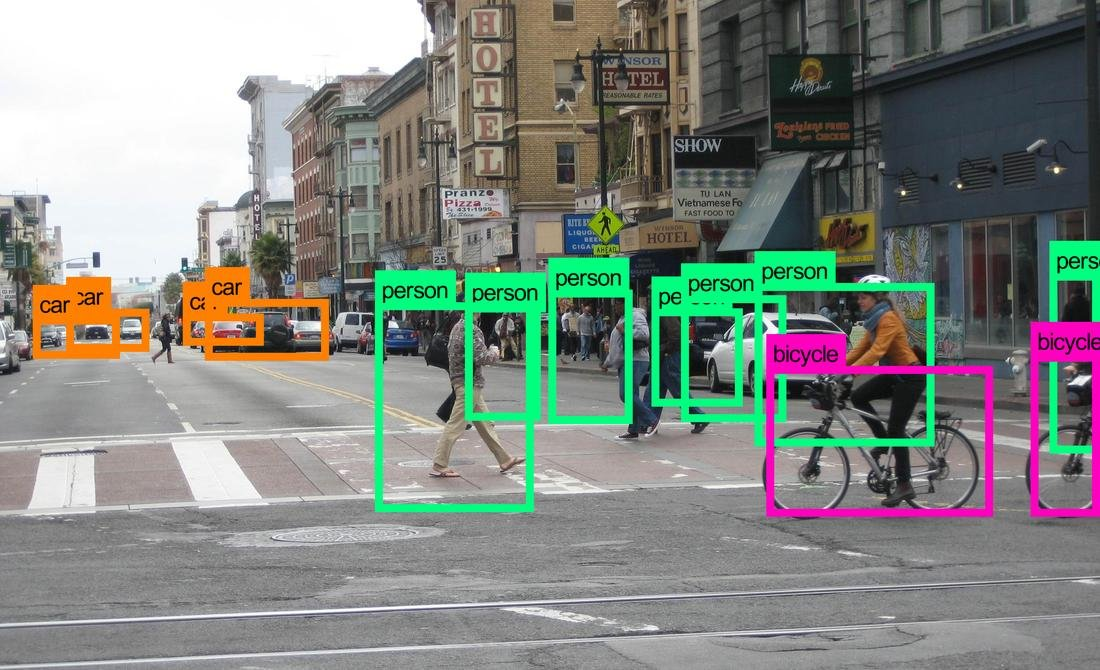
\includegraphics[width=0.68\textwidth]{dectection_dobjet_en_utilisant_regions_avec_cnn.jpg}
  \caption{Détection d'objets par réseau à régions (R-CNN), hors du périmètre de notre projet}
  \label{fig:detection}
\end{figure}

\section{Besoins fonctionnels}
\label{sec:besoins-fonctionnels}

Les besoins fonctionnels regroupent l'ensemble des fonctionnalités que le système doit offrir. Les exigences EF01 à EF06 reprennent les attentes du sujet, tandis que les exigences EF07 à EF14 concernent l'intégration dans le véhicule virtuel. Pour chacune d'elles, nous avons défini un critère d'acceptation qui permettra de vérifier qu'elle est remplie.

\begin{table}[H]
\centering
\small
\caption{Exigences fonctionnelles consolidées}
\begin{tabularx}{\textwidth}{l>{\raggedright\arraybackslash}p{5.4cm}Y}
  \toprule
  \entete \textbf{ID} & \textbf{Exigence} & \textbf{Critère d'acceptation} \\
  \midrule
  EF01 & Charger et explorer le dataset routier & Effectifs par classe, tailles et exemples présentés (notebook 01) \\
  EF02 & Prétraiter les images & Images filtrées, recadrées, redimensionnées et normalisées, découpage sans photo partagée (notebook 02) \\
  EF03 & Extraire les caractéristiques visuelles & Descripteurs HOG calculés pour toutes les images (notebook 03) \\
  EF04 & Entraîner plusieurs modèles de classification & SVM, Random Forest et k-NN entraînés sur les mêmes caractéristiques \\
  EF05 & Évaluer et comparer les modèles & Tableau commun : accuracy, précision, rappel, F1 et matrices de confusion \\
  EF06 & Prédire la classe d'un nouvel objet & Une image inconnue donne une classe et un score affichés \\
  EF07 & Récupérer les coordonnées des objets dans le simulateur & Chaque obstacle possède un tronçon de rue et une position sur ce tronçon \\
  EF08 & Associer les prédictions aux objets virtuels & Chaque prédiction est rattachée à l'obstacle dont provient l'image \\
  EF09 & Représenter les obstacles dans l'environnement & Tronçons bloqués ou pénalisés selon la décision \\
  EF10 & Calculer le chemin vers la destination avec Dijkstra & Plus court chemin trouvé sur la carte et vérifié par des tests \\
  EF11 & Adapter le trajet en présence d'un obstacle & Nouveau calcul après chaque obstacle bloquant \\
  EF12 & Décider de ralentir, s'arrêter ou contourner & Une action par classe prédite, et un arrêt prudent si le score est trop faible \\
  EF13 & Commander le véhicule virtuel & Le véhicule avance, ralentit, s'arrête, fait demi-tour ou change de rue \\
  EF14 & Afficher les prédictions et les décisions du véhicule & Image, classe, score et action visibles à l'écran \\
  \bottomrule
\end{tabularx}
\end{table}

\section{Besoins non fonctionnels}

Les besoins non fonctionnels définissent les critères de qualité et les contraintes que le système doit respecter. Ils ne concernent pas directement les fonctionnalités visibles, mais influencent fortement la fiabilité des résultats et la crédibilité du projet.

\begin{itemize}
  \item \textbf{Entraînement de zéro}\\
  Aucun YOLO, aucun détecteur et aucun poids préentraîné ne doivent être utilisés dans notre modèle.
  \item \textbf{Fiabilité de l'évaluation}\\
  Le découpage doit se faire par photo d'origine, et le jeu de test ne doit être utilisé qu'une seule fois, lors de l'évaluation finale.
  \item \textbf{Reproductibilité}\\
  Les graines aléatoires doivent être fixées, les essais notés, et les notebooks exécutables de bout en bout.
  \item \textbf{Cohérence du prétraitement}\\
  La taille des images, l'ordre des couleurs et la normalisation doivent être identiques dans les notebooks et dans le simulateur.
  \item \textbf{Séparation entre vérité terrain et perception}\\
  Les décisions du véhicule ne doivent jamais utiliser la vraie classe connue du simulateur, mais uniquement la classe prédite par le modèle.
  \item \textbf{Honnêteté des résultats}\\
  Aucune métrique ne doit être inventée. Sans modèle chargé, l'interface doit afficher \og SIMULATION --- modèle réel non chargé \fg{}.
  \item \textbf{Respect des licences}\\
  Les sources des données (COCO), de la carte (OpenStreetMap, licence ODbL) et des illustrations doivent être citées.
  \item \textbf{Temps de réponse}\\
  Une prédiction doit prendre quelques millisecondes sur un processeur ordinaire, afin de garantir une démonstration fluide.
\end{itemize}

\section{Contraintes techniques et académiques}

Le projet doit respecter plusieurs contraintes, liées à la fois au cadre du cours et aux moyens dont dispose l'équipe :

\begin{itemize}
  \item \textbf{Règles du cours}\\
  L'utilisation de YOLO, de détecteurs et de poids préentraînés est interdite pour notre modèle. Les classifieurs à comparer sont ceux du sujet : SVM, Random Forest et k-NN.
  \item \textbf{Calendrier}\\
  Le projet s'organise autour de trois échéances fixes : la séance 1 le 4 novembre, la séance 2 le 25 novembre et la soutenance le 16 décembre 2026.
  \item \textbf{Matériel}\\
  Aucun membre de l'équipe ne dispose d'un GPU. Les traitements doivent donc pouvoir s'exécuter sur un processeur ordinaire, avec le GPU gratuit de Google Colab en appui.
  \item \textbf{Budget}\\
  Le projet ne nécessite aucun budget, car l'ensemble des outils et des données retenus sont gratuits.
  \item \textbf{Licences}\\
  Les images de COCO conservent leur licence Flickr et ne sont donc pas redistribuées dans le dépôt Git.
\end{itemize}

\begin{table}[H]
\centering
\small
\caption{Ressources nécessaires au projet}
\begin{tabularx}{\textwidth}{>{\raggedright\arraybackslash}p{2.6cm}Y>{\raggedright\arraybackslash}p{4.4cm}}
  \toprule
  \entete \textbf{Ressource} & \textbf{Détail} & \textbf{Solution} \\
  \midrule
  Données & Images des 6 classes, étiquettes fiables, licence compatible & COCO 2017, à valider par l'encadrante \\
  Calcul & Entraînement des modèles & Processeur local, Google Colab en appui \\
  Stockage & Données, poids et figures partagés & Dossier Google Drive partagé \\
  Poste local & Fenêtre du simulateur, que Colab ne peut pas ouvrir & Disponible \\
  Encadrement & Validation du dataset et du périmètre & Section~\ref{sec:criteres-go} \\
  \bottomrule
\end{tabularx}
\end{table}

\section{Méthodologie et planning prévisionnel}

Pour la conduite de ce projet, nous avons retenu une démarche en \textbf{deux phases}, illustrée par la figure~\ref{fig:flux}. La première phase consiste à développer et à entraîner le modèle dans des notebooks versionnés sur GitHub. La seconde consiste à charger le modèle exporté dans le simulateur, sans jamais l'y réentraîner.

\begin{figure}[H]
  \centering
  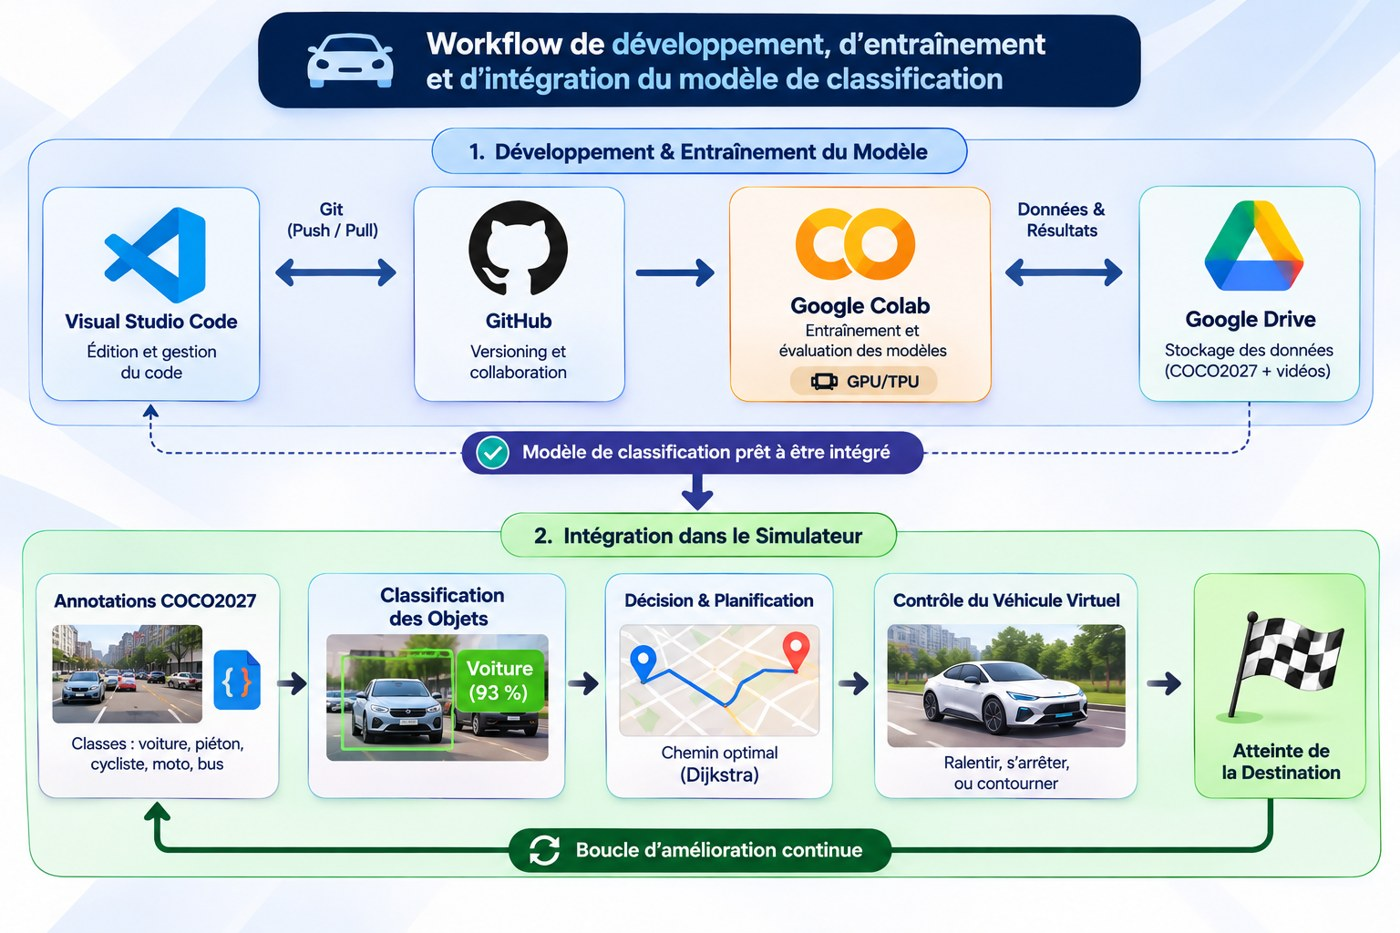
\includegraphics[width=0.9\textwidth]{flux_de_developpement_et_integration_autonome.jpg}
  \caption{Flux de développement, d'entraînement et d'intégration du modèle (lire COCO 2017, classes complétées par le camion)}
  \label{fig:flux}
\end{figure}

Cette démarche s'organise en quatre grandes étapes :

\begin{enumerate}
  \item \textbf{Données (notebooks 01 et 02)} : acquisition, exploration, nettoyage, recadrage et découpage des images.
  \item \textbf{Modèles (notebook 03)} : extraction des descripteurs HOG, puis entraînement et réglage de SVM, Random Forest et k-NN sur le jeu de validation.
  \item \textbf{Évaluation (notebook 05)} : mesure unique sur le jeu de test, analyse des erreurs et prédiction sur de nouvelles images.
  \item \textbf{Intégration} : export du modèle, branchement dans le simulateur et comparaison sur plusieurs épisodes de conduite.
\end{enumerate}

Sur le plan de l'organisation, une seule personne modifie un notebook à la fois, et chaque notebook est relu par un autre membre avant chaque séance. Les décisions importantes sont consignées dans un journal de bord. Le planning détaillé est présenté à la section~\ref{sec:planning}.

\section{Conclusion}

Ce premier chapitre a permis de définir le \textbf{cadre général du projet AutoMaze AI} en précisant son contexte, sa problématique, ses objectifs et son périmètre. L'élaboration du cahier des charges a constitué une étape essentielle pour traduire les attentes du sujet en exigences vérifiables, tout en distinguant clairement le travail de Machine Learning, qui reste au cœur du projet, des fonctionnalités d'intégration. Cette analyse préliminaire servira de base au chapitre suivant, consacré à l'analyse fonctionnelle et à la conception du système.
